\documentclass[16pt]{beamer}

\ifdefined\chinchin
\usepackage[CJKspace]{xeCJK}
%\setCJKmainfont[BoldFont=SimHei,ItalicFont=AR PL KaitiM GB]{Alibaba PuHuiTi}
\setCJKmainfont{Alibaba PuHuiTi}
\newcommand{\cc}[2]{#1}
\else
\newcommand{\cc}[2]{#2}
\fi

%\usepackage{newtxtext,newtxmath}	% use Times Roman font
%\usepackage{newtxtext}
%\renewcommand{\familydefault}{\sfdefault}
%\usefonttheme{serif}
\usefonttheme{professionalfonts}
%\setbeamertemplate{theorems}[numbered]
\setbeamertemplate{caption}{\insertcaption} 	% no `Figure' prefix before caption

\mode<presentation> {

%\usetheme{default}
%\usetheme{AnnArbor}
%\usetheme{Antibes}
%\usetheme{Bergen}
%\usetheme{Berkeley}
%\usetheme{Berlin}
%\usetheme{Boadilla}
%\usetheme{CambridgeUS}
%\usetheme{Copenhagen}
%\usetheme{Darmstadt}
%\usetheme{Dresden}
%\usetheme{Frankfurt}
%\usetheme{Goettingen}
%\usetheme{Hannover}
%\usetheme{Ilmenau}
%\usetheme{JuanLesPins}
%\usetheme{Luebeck}
\usetheme{Madrid}
%\usetheme{Malmoe}
%\usetheme{Marburg}
%\usetheme{Montpellier}
%\usetheme{PaloAlto}
%\usetheme{Pittsburgh}
%\usetheme{Rochester}
%\usetheme{Singapore}
%\usetheme{Szeged}
%\usetheme{Warsaw}

%\usecolortheme{albatross}
%\usecolortheme{beaver}
%\usecolortheme{beetle}
%\usecolortheme{crane}
%\usecolortheme{dolphin}
%\usecolortheme{dove}
%\usecolortheme{fly}
%\usecolortheme{lily}
\usecolortheme{orchid}
%\usecolortheme{rose}
%\usecolortheme{seagull}
%\usecolortheme{seahorse}
%\usecolortheme{whale}
%\usecolortheme{wolverine}		% Hofstra

%\setbeamertemplate{footline} % To remove the footer line in all slides uncomment this line
\setbeamertemplate{footline}[page number] % To replace the footer line in all slides with a simple slide count uncomment this line
\setbeamertemplate{navigation symbols}{} % To remove the navigation symbols from the bottom of all slides uncomment this line
}

\setbeamertemplate{headline}{}
\setbeamersize{text margin left=1mm,text margin right=1mm} 
\settowidth{\leftmargini}{\usebeamertemplate{itemize item}}
\addtolength{\leftmargini}{\labelsep}

\usepackage[backend=biber,style=numeric]{biblatex}
\bibliography{../AGI-book}
% \renewcommand*{\bibfont}{\footnotesize}
\setbeamertemplate{bibliography item}[text]

\usepackage{graphicx} % Allows including images
\usepackage{tikz-cd}
\usepackage{tikz}
\usepackage[export]{adjustbox}% http://ctan.org/pkg/adjustbox
\usepackage{verbatim} % comments
% \usepackage{tikz-cd}  % commutative diagrams
% \newcommand{\tikzmark}[1]{\tikz[overlay,remember picture] \node (#1) {};}
% \usepackage{booktabs} % Allows the use of \toprule, \midrule and \bottomrule in tables
% \usepackage{amssymb}  % \leftrightharpoons
% \usepackage{wasysym} % frownie face
% \usepackage{newtxtext,newtxmath}	% Times New Roman font
% \usepackage{sansmath}

\newcommand{\emp}[1]{{\color{violet}#1}}
\newcommand{\vect}[1]{\boldsymbol{#1}}
\newcommand{\tab}{\hspace*{1cm}}
\newcommand*\confoundFace{$\vcenter{\hbox{\includegraphics[scale=0.2]{../confounded-face.jpg}}}$}
\newcommand{\smiley}{$\vcenter{\hbox{\includegraphics[scale=0.05]{../smiling-face.png}}}$}

%%%%%%%% Make table of contents %%%%%%%

\makeatletter
\renewcommand{\boxed}[1]{\fbox{\m@th$\displaystyle\scalebox{0.9}{#1}$} \,}
\makeatother
\newif\ifframeinlbf
\frameinlbftrue
\makeatletter
\newcommand\listofframes{\@starttoc{lbf}}
\makeatother
\addtobeamertemplate{frametitle}{}{%
	\ifframeinlbf
	\addcontentsline{lbf}{section}{\protect\makebox[2em][l]{%
			\protect\usebeamercolor[fg]{structure}\insertframenumber\hfill}%
		\insertframetitle\par}%
	\else\fi
}

%----------------------------------------------------------------------------------------
%	TITLE PAGE
%----------------------------------------------------------------------------------------

\title[Logic route to strong AI]{{\Huge《The logic route to strong AI》} \\ \vspace*{0.4cm} Alibaba HKAI Lab 2020 presentation}
\author{\cc{Heelal team}{Heelal team}} % Your name
%\institute[] % Your institution as it will appear on the bottom of every slide, may be shorthand to save space
%{
%Independent researcher, Hong Kong \\ % Your institution for the title page
%\medskip
%\textit{generic.intelligence@gmail.com} % Your email address
%}
\date{\today} % Date, can be changed to a custom date

\begin{document}

\frameinlbffalse
\addtocounter{page}{-1}
\begin{frame}[plain,noframenumbering]
\titlepage
\end{frame}

\addtocounter{page}{-1}
\begin{frame}[noframenumbering]
\frametitle{Table of contents}
\listofframes
% \vspace*{0.5cm}
% 多谢 支持 \smiley
\end{frame}

%----------------------------------------------------------------------------------------
%	PRESENTATION SLIDES
%----------------------------------------------------------------------------------------

%------------------------------------------------

\frameinlbftrue

\begin{frame}
\frametitle{CNN 在机器视觉中的成功}
\begin{itemize}
	\item 在几何学上,视觉 具有 \emp{平移 不变性}:
	\begin{equation}
	\vcenter{\hbox{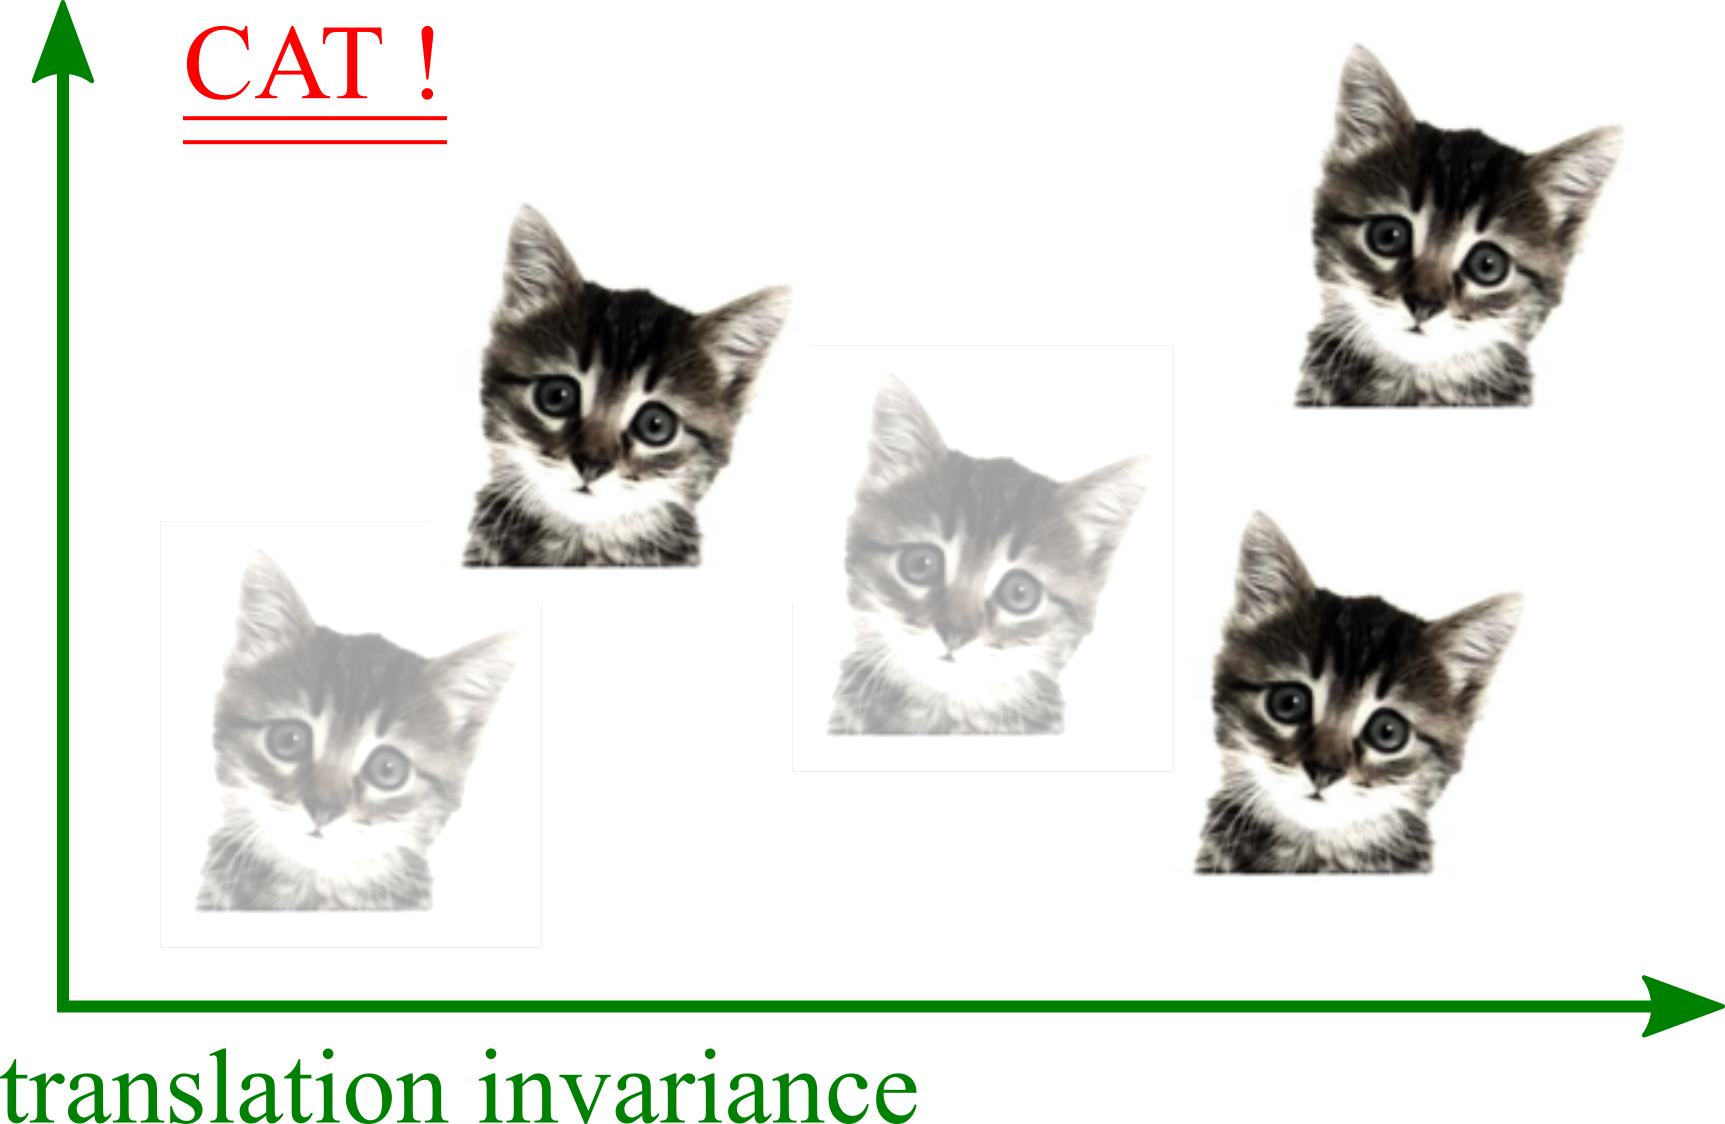
\includegraphics[scale=0.5]{translation-invariance.png}}}
	\end{equation}
	\item Convolution 是一种具有平移不变性的运算:
	\begin{equation}
	(T_x \circ f) * g = T_x \circ ( f * g )
	\end{equation}
	\item Yann LeCun 等人 利用 CNN 的 \emp{对称性} 加快了学习速度,成功地解决了 机器视觉 的问题
\end{itemize}
\end{frame}

\begin{frame}
\frametitle{Symmetry and inductive bias}
\begin{itemize}
	\item 在数学上,\emp{对称性} 经常能简化计算,所以数学家 特别喜欢 对称
	\item 在机器学习中,经常要引入 归纳偏好 (inductive bias),缩小 \emp{搜寻空间}:
	\begin{equation}
	\vcenter{\hbox{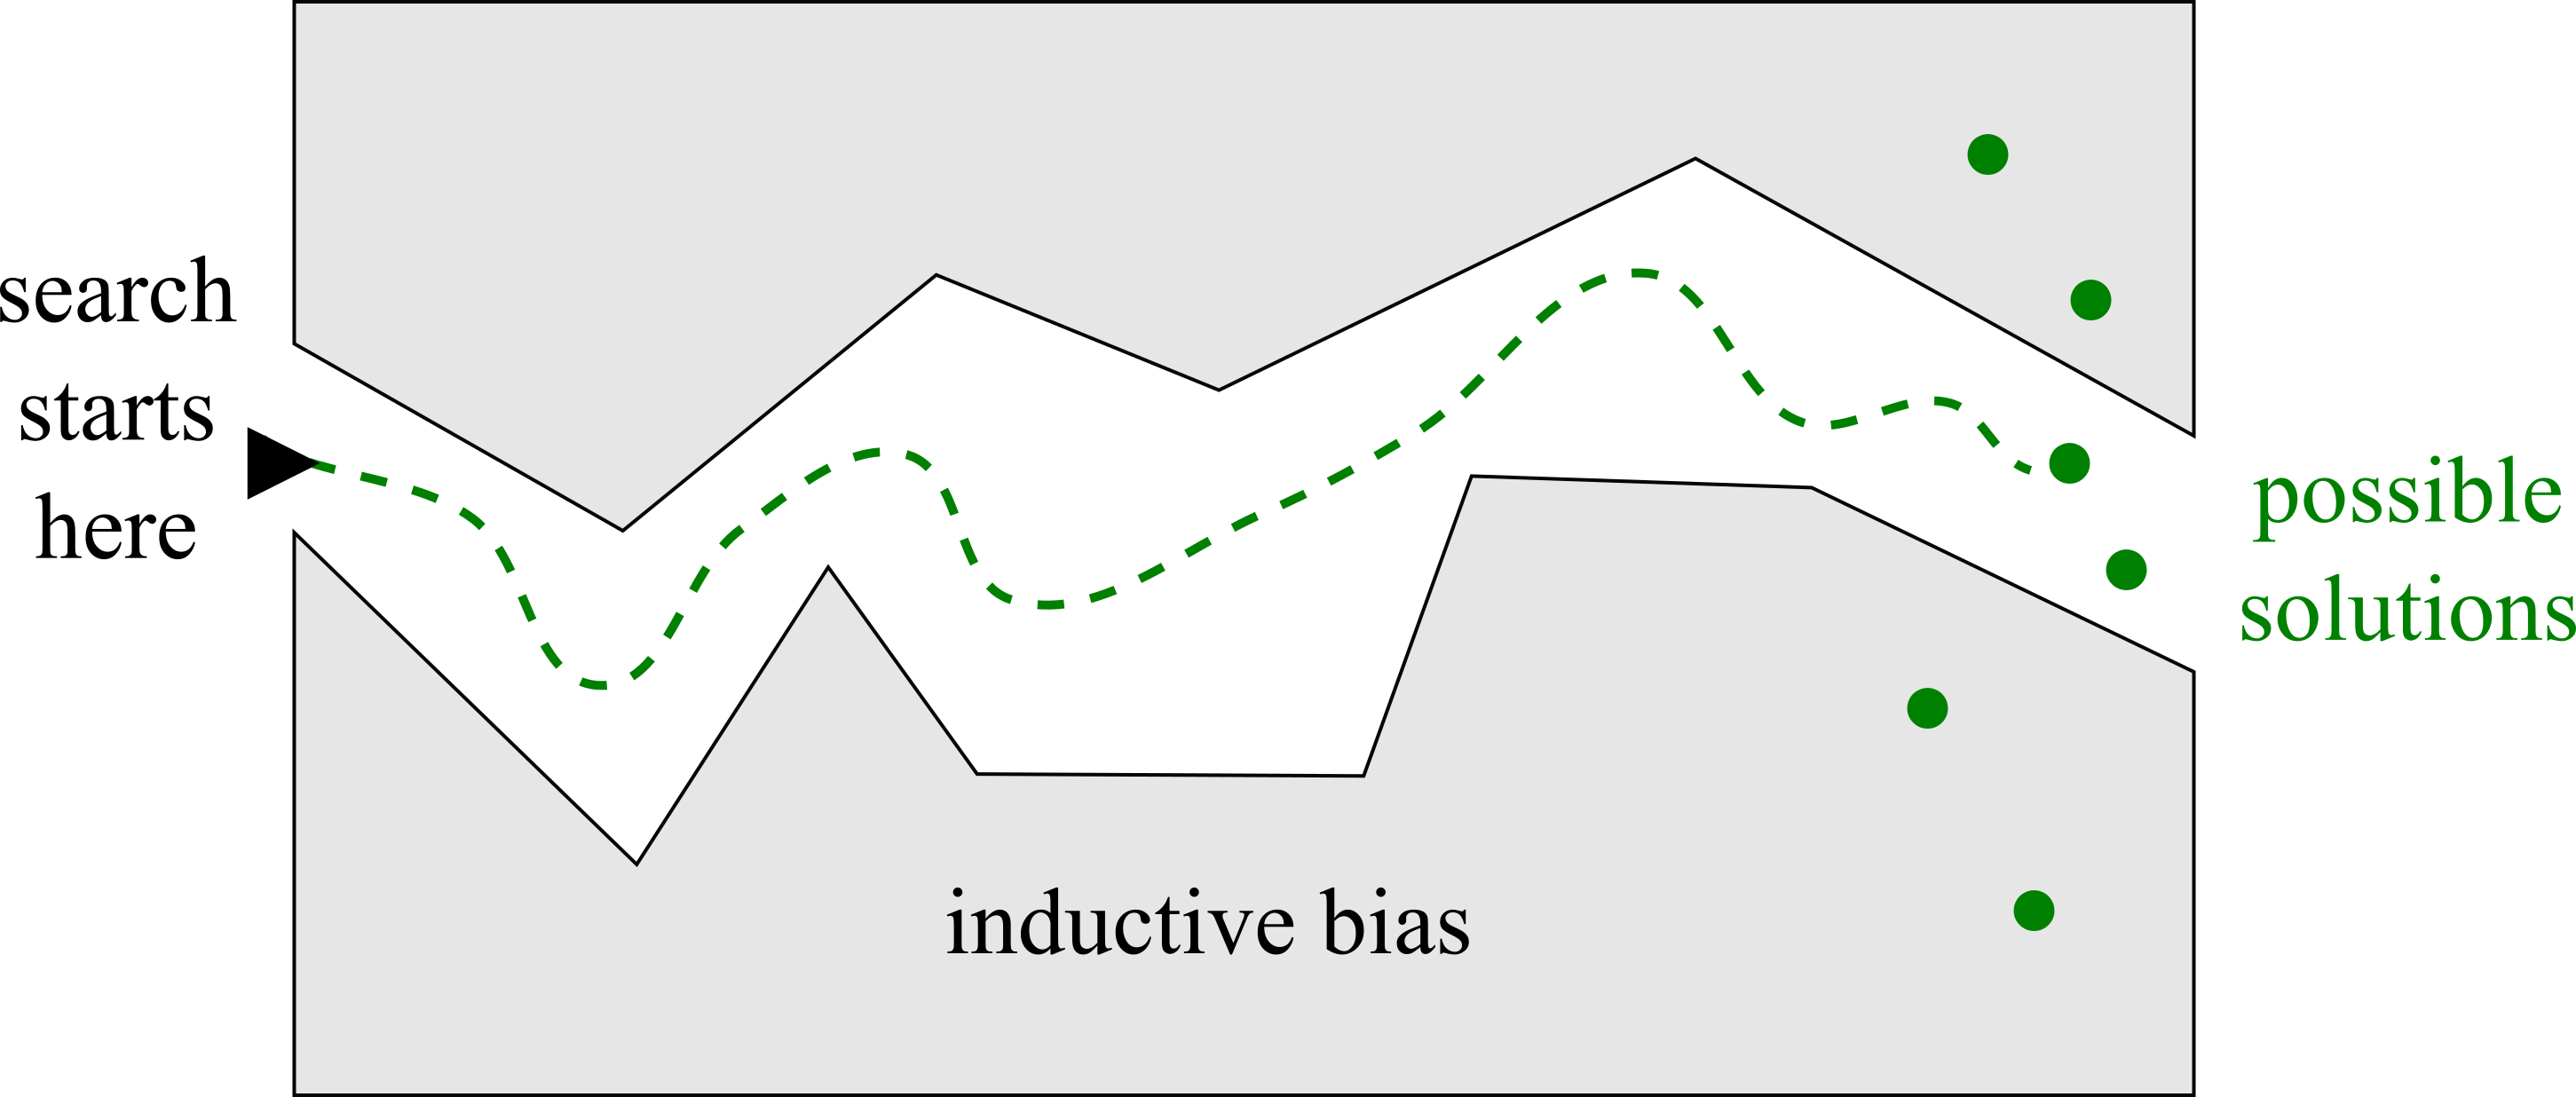
\includegraphics[scale=0.5]{no-free-lunch.png}}}
	\end{equation}
	\item 往往如果 归纳偏好 选对了,可以在短时间内找到答案,否则问题是不可解的 (intractable)
\end{itemize}
\end{frame}

\begin{frame}
\frametitle{Richard Sutton 的观点}
\begin{itemize}
	\item Richard Sutton 认为,我们只需在 强化学习 的框架下 \emp{增加计算力},就可以找到 strong AI
	\item 下面描述的只是众多 形式逻辑 之中可能的一种:
	\begin{equation}
	\vcenter{\hbox{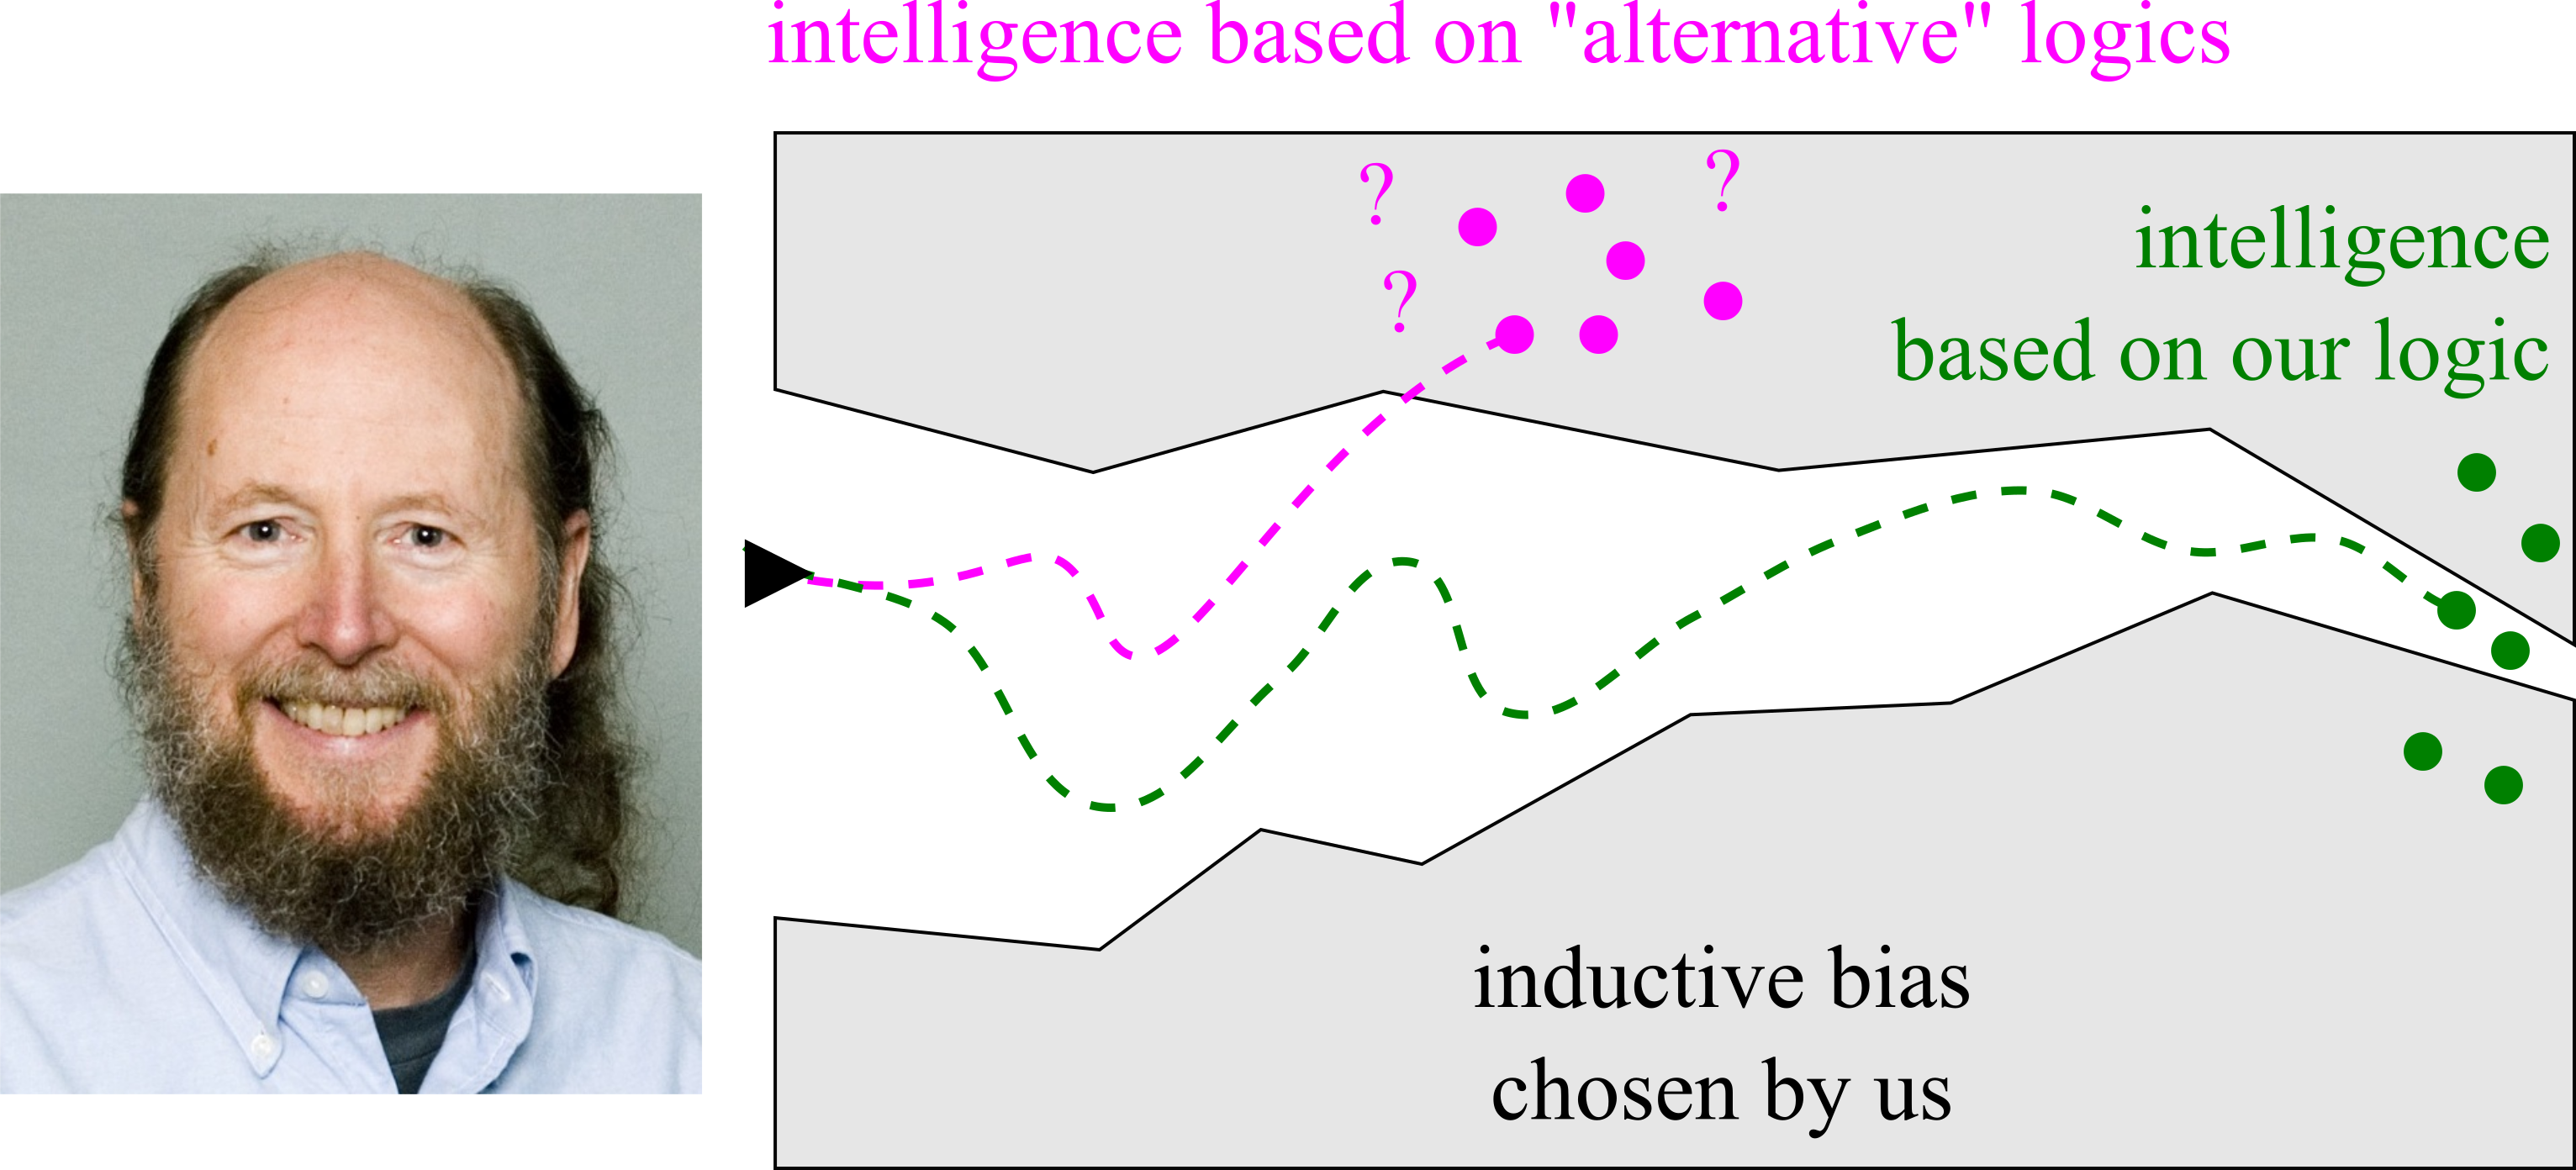
\includegraphics[scale=0.5]{no-free-lunch_Richard-Sutton.png}}}
	\end{equation}
	\item 这不只是一个「空想」的问题; 事实上,世界各地的实验室 已经开始了对 AGI 不同形式的搜索!
\end{itemize}
\end{frame}

\begin{frame}
\frametitle{对 逻辑主义 的质疑}
\begin{itemize}
	\item 很多人怀疑: 人脑真的用 逻辑 思考吗?
	\item 其实我们每句表达的 \emp{语言},都是逻辑形式的 (logical form)
	\item 直觉认为,人脑 构造一些 \emp{models},再从 model 中「读出」一些结论
	\item 例如给定一个描述:「已婚妇人出轨,用刀刺死丈夫」
	\begin{equation}
	\vcenter{\hbox{
\includegraphics[scale=1.0]{murder-scene.png}}}
	\end{equation}
	\item 那么 妻子穿著什么衣服? 衣服什么颜色? 
	\item 这个 model 可以有哪些细节? 答案是: 任何细节都不可以有,除非是 逻辑上蕴含的
	\item 其实人脑可能比我们想像中更接近逻辑化的结构
\end{itemize}
\end{frame}

\begin{frame}
\frametitle{Structure of logic}
\begin{itemize}
	\item 我的想法是: 在深度学习中引入 \emp{逻辑} 的对称性,解决 strong AI 问题
	\item 因为人的思维 具有 逻辑 的结构,这个 inductive bias 可以帮助我们快速找到 the solution to strong AI
	\item 逻辑结构很复杂,但最粗略的 symmetry 是 命题的 \emp{可交换律} (commutativity, or permutation invariance):
	\begin{equation}
	\begin{aligned}
	A &\wedge B & \equiv && B & \wedge A \\
	\mbox{下雨} &\wedge \mbox{失恋} & \equiv && \mbox{失恋} &\wedge \mbox{下雨}
	\end{aligned}
	\end{equation}
	\item 它的重要性类似於 视觉中的 平移不变性
	\item 另一种讲法是: 它将智能系统的 \emp{思维状态} (mental state) 分拆成 一粒粒独立的 \emp{命题} (propositions)
\end{itemize}
\end{frame}

\begin{frame}
\frametitle{Symmetric neural networks}
\begin{itemize}
	\item Permutation invariance can be handled by \emp{symmetric} neural networks

	\item \cc{我浪费了两年时间试图解决这问题,却发现在3年前已经有两篇论文解决了 [PointNet 2017] [DeepSets 2017],而且数学水平比我高很多!
	}
	{I wasted 2 years trying to solve this problem, but found out that it has been solved 3 years ago:  [PointNet 2017] and [DeepSets 2018] and their mastery of mathematics is significantly above me!}

	\item Any symmetric function can be represented by the following form (a special case of the Kolmogorov-Arnold representation of functions):
	\begin{equation}
	f(x, y, ...) = g(h(x) + h(y) + ... )
	\end{equation}
	\begin{equation}
	\vcenter{\hbox{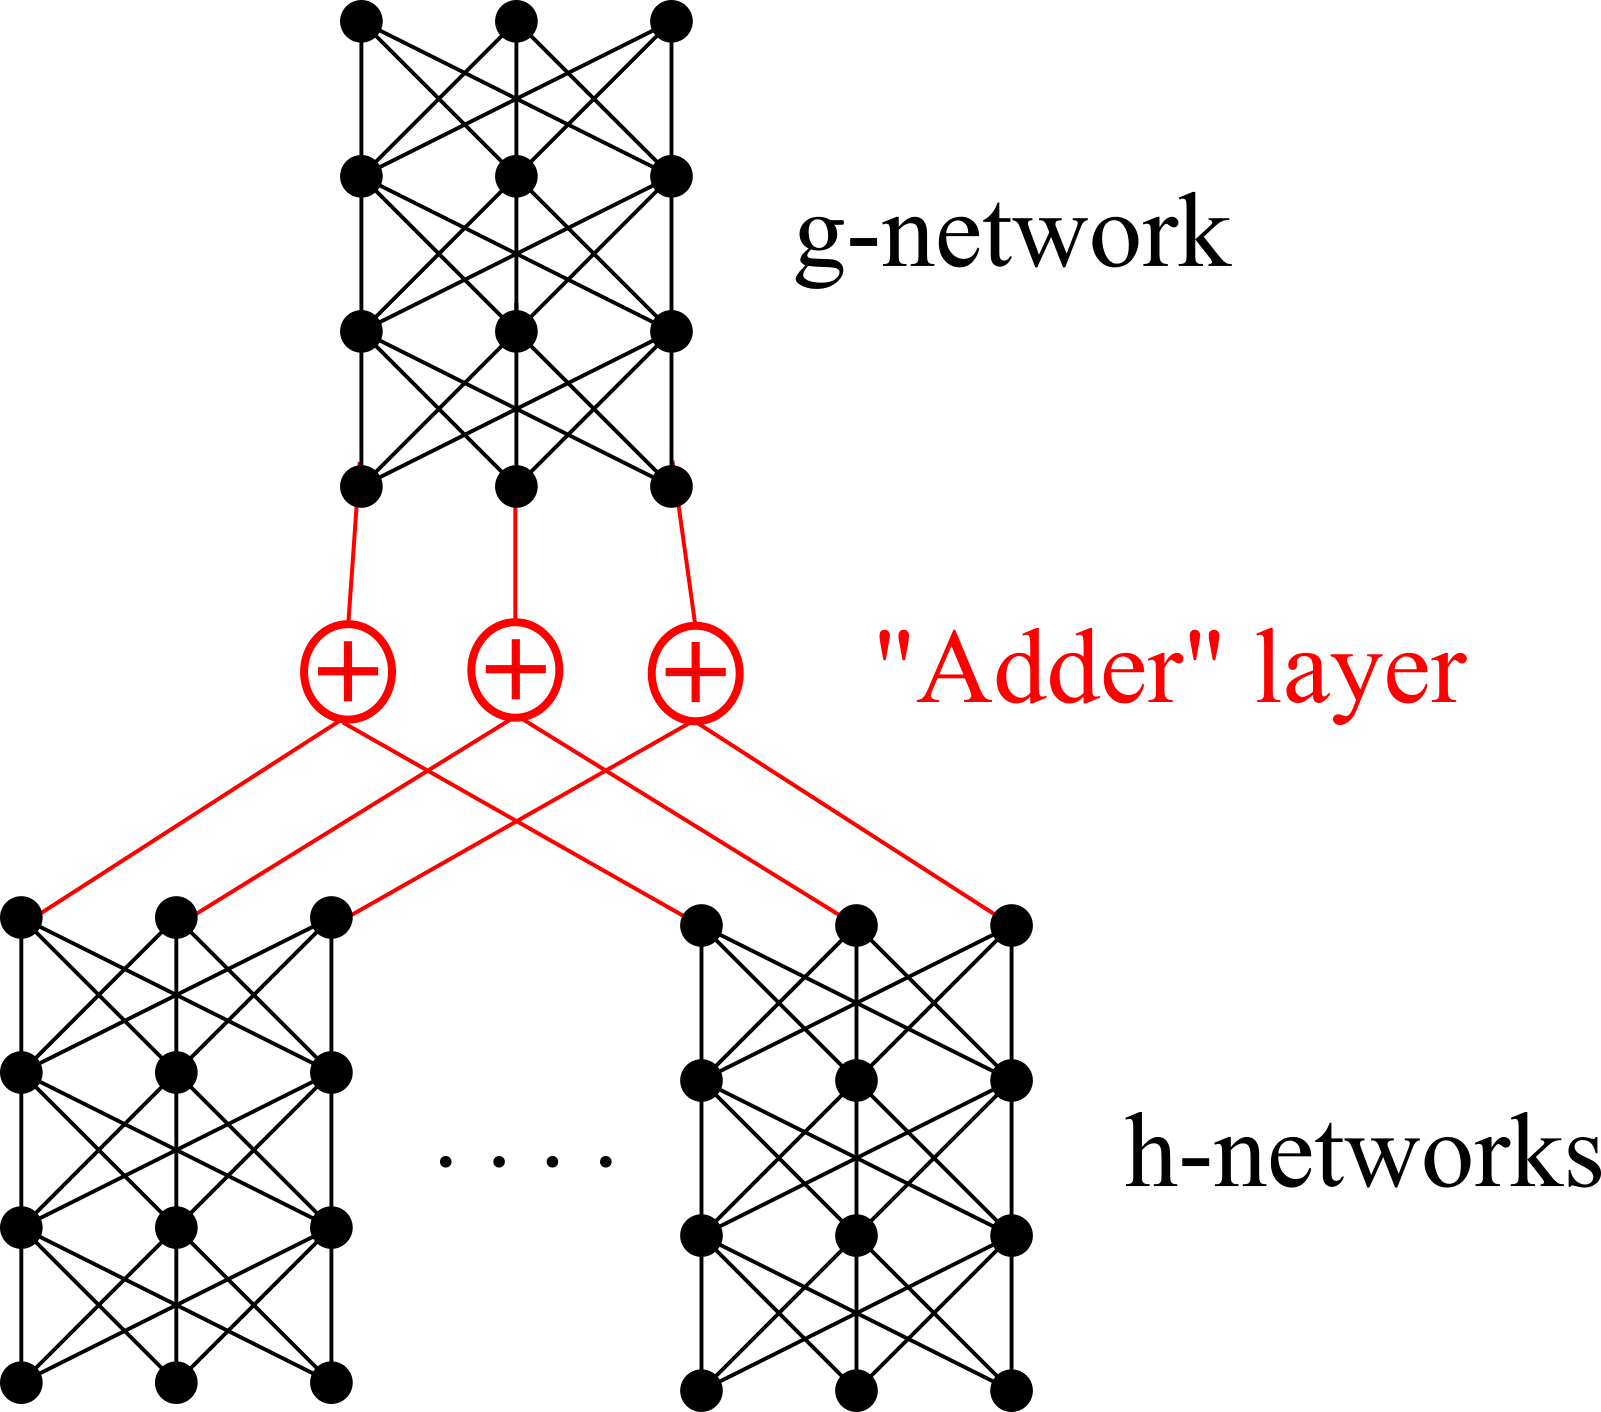
\includegraphics[scale=0.5]{g-and-h-networks.png}}}
	\end{equation}
\end{itemize}
\nocite{Qi2017a}
\nocite{Zaheer2017}
\end{frame}

\begin{frame}[plain]
\begin{itemize}
	\item Sym NN gives a powerful boost in efficiency $\propto n!$ where $n = \# \mbox{inputs}$

	\item The code for Sym NN is just a few lines of Tensorflow:
	\begin{equation}
	\vcenter{\hbox{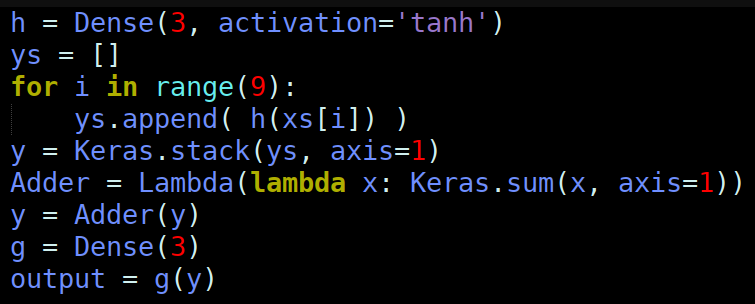
\includegraphics[scale=0.4]{sym-NN-code.png}}}
	\end{equation}
	\item Very easy to adopt this to existing models such as BERT and reinforcement learning
	\item I have successfully tested it on the game of TicTacToe
\end{itemize}
\end{frame}

\begin{frame}
\frametitle{应用:知识图谱 (knowledge graphs)}
\begin{itemize}
	\item 知识图谱 不能直接输入神经网络,它必需分拆成很多 edges,每个 edge 是一个 \emp{关系},也是一个 \emp{逻辑命题} ;也可以说 ``graphs are isomorphic to logic''
	\begin{equation}
	\vcenter{\hbox{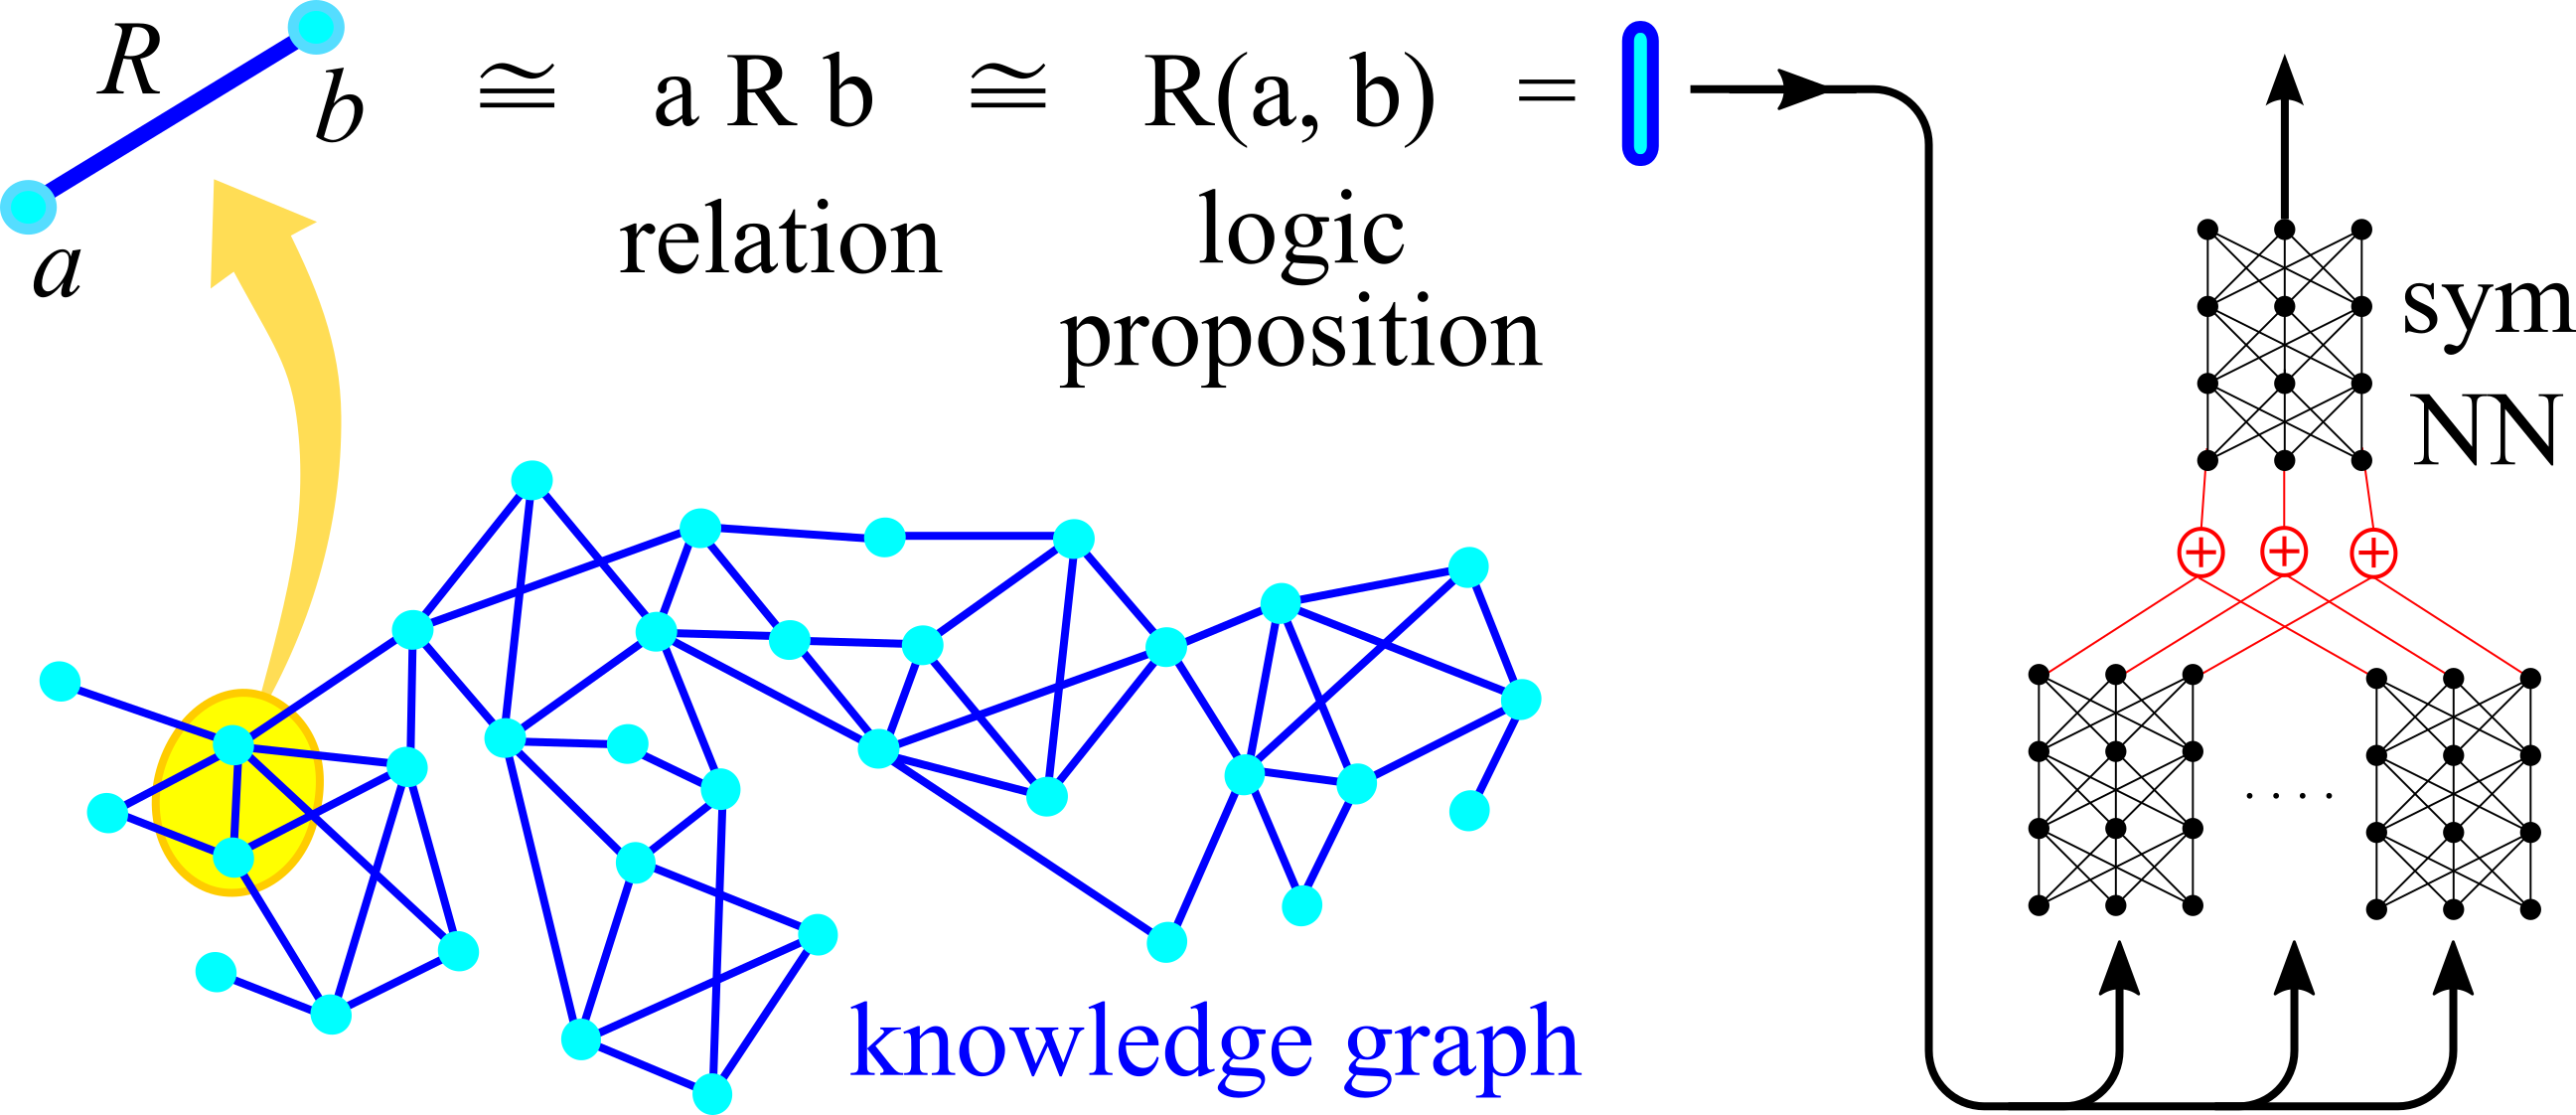
\includegraphics[scale=0.6]{knowledge-graph.png}}}
	\end{equation}
	\item 而这些 edges 似乎必需用 \emp{symmetric} NN 处理,因为它们是 permutation invariant
	% \item Sym NNs are required to handle \emp{graph-rewriting}, an essential operation on knowledge graphs
\end{itemize}
\end{frame}

\begin{frame}
\frametitle{\cc{应用:BERT 的逻辑化}{Logicalization of BERT}}
\begin{itemize}
	\item 类似地,可以将 BERT 的 隐状态 变成 ``set of propositions'' 的形式,方法是将 原来的 decoder 变成 sym NN:
	\begin{equation}
	\vcenter{\hbox{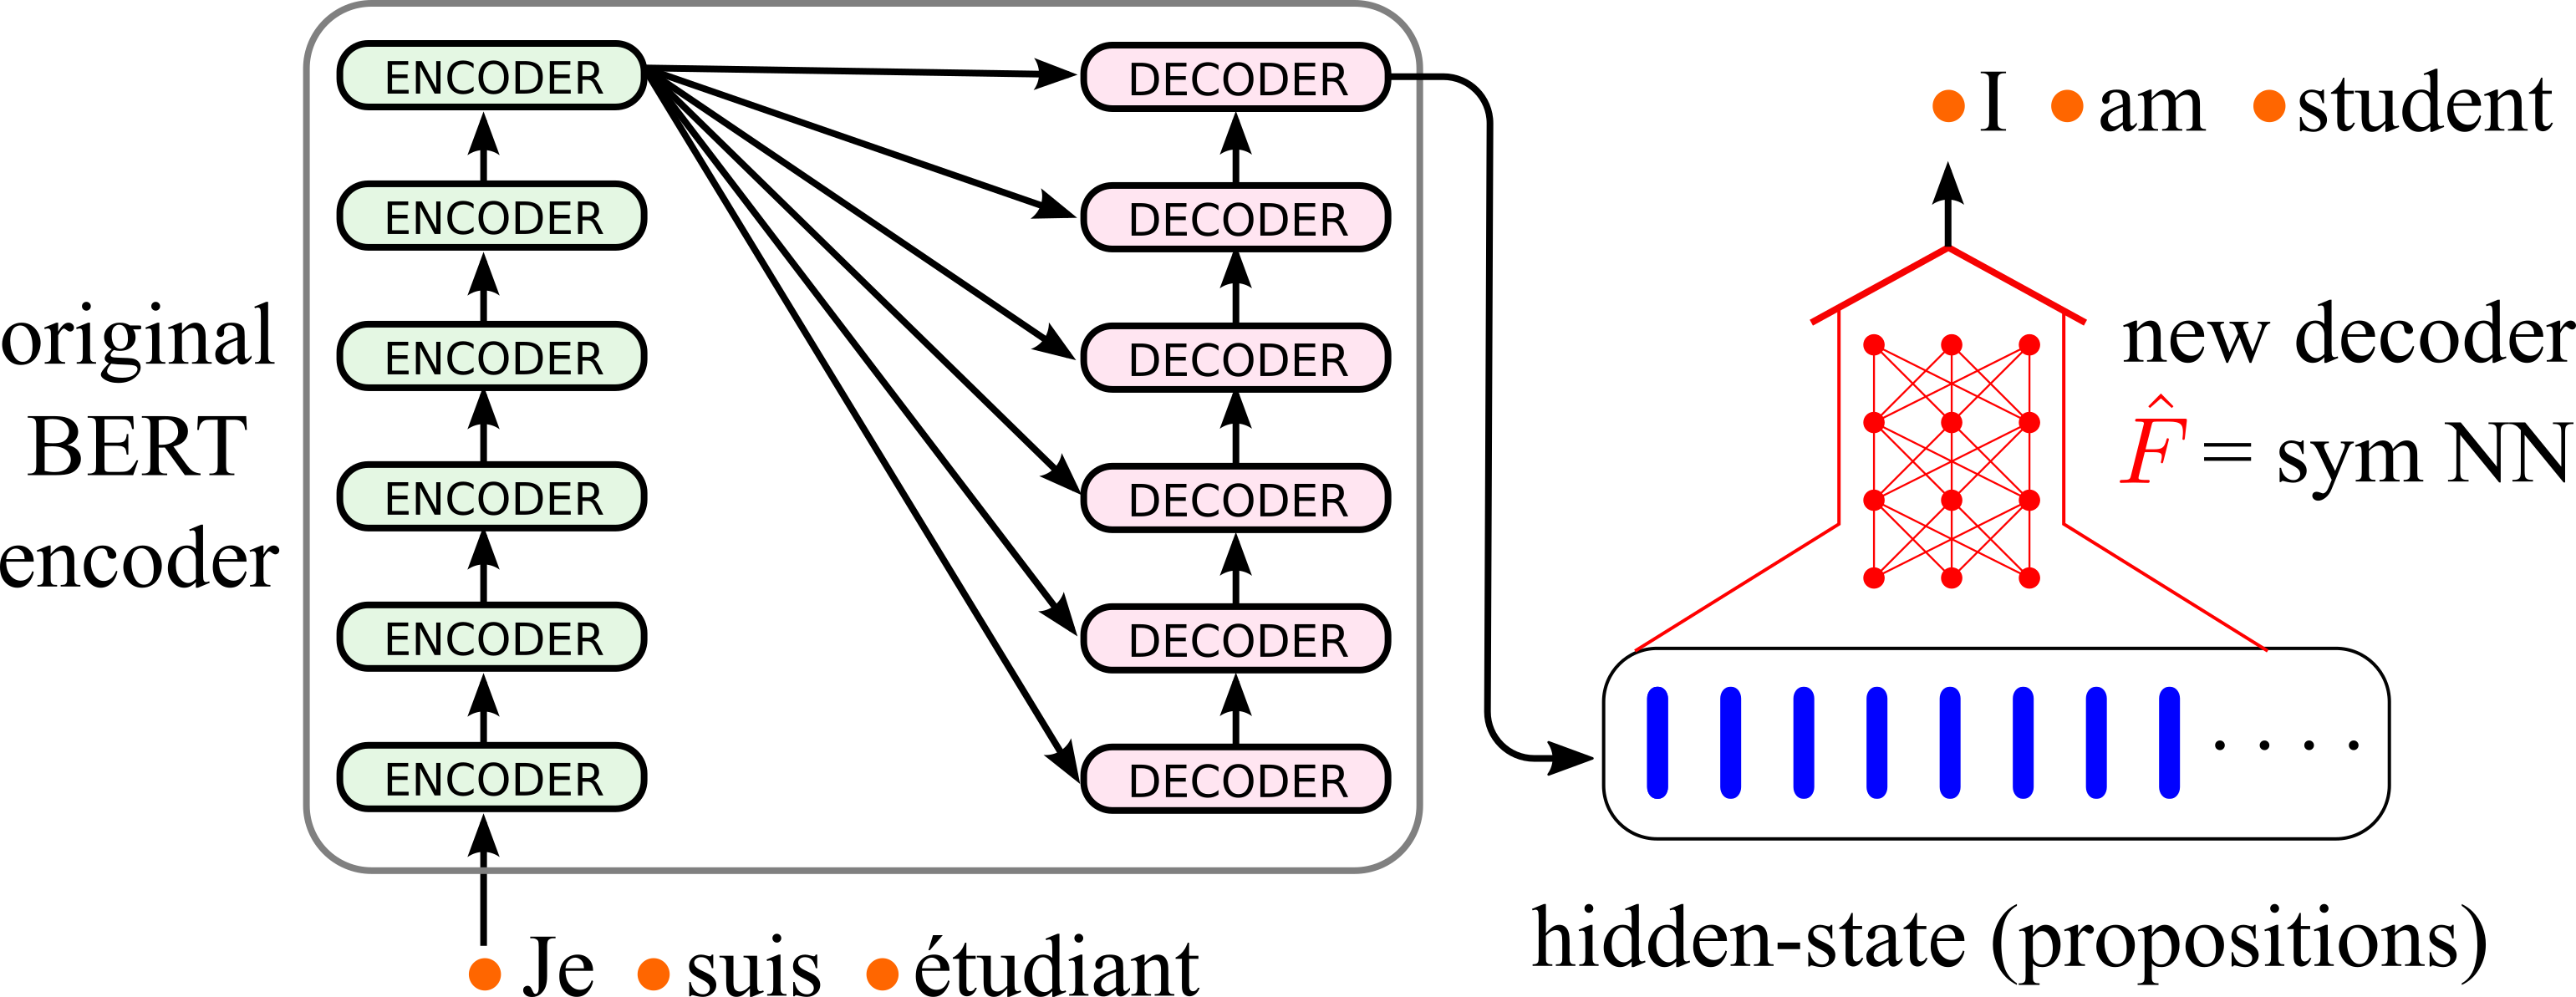
\includegraphics[scale=0.6]{new-BERT.png}}}
	\end{equation}
	\item 原来的 encoder 可以照旧使用,因为后半部改变了,error propagation 会令 representation 也改变
	\item 当然,这个想法有待实验证实 \smiley
\end{itemize}
\end{frame}

\begin{frame}
\frametitle{应用:content-addressable long-term memory}
\begin{itemize}
	\item 将 BERT 的内部状态 逻辑化之后,可以储存在 \emp{长期记忆} 中:
	\begin{equation}
	\vcenter{\hbox{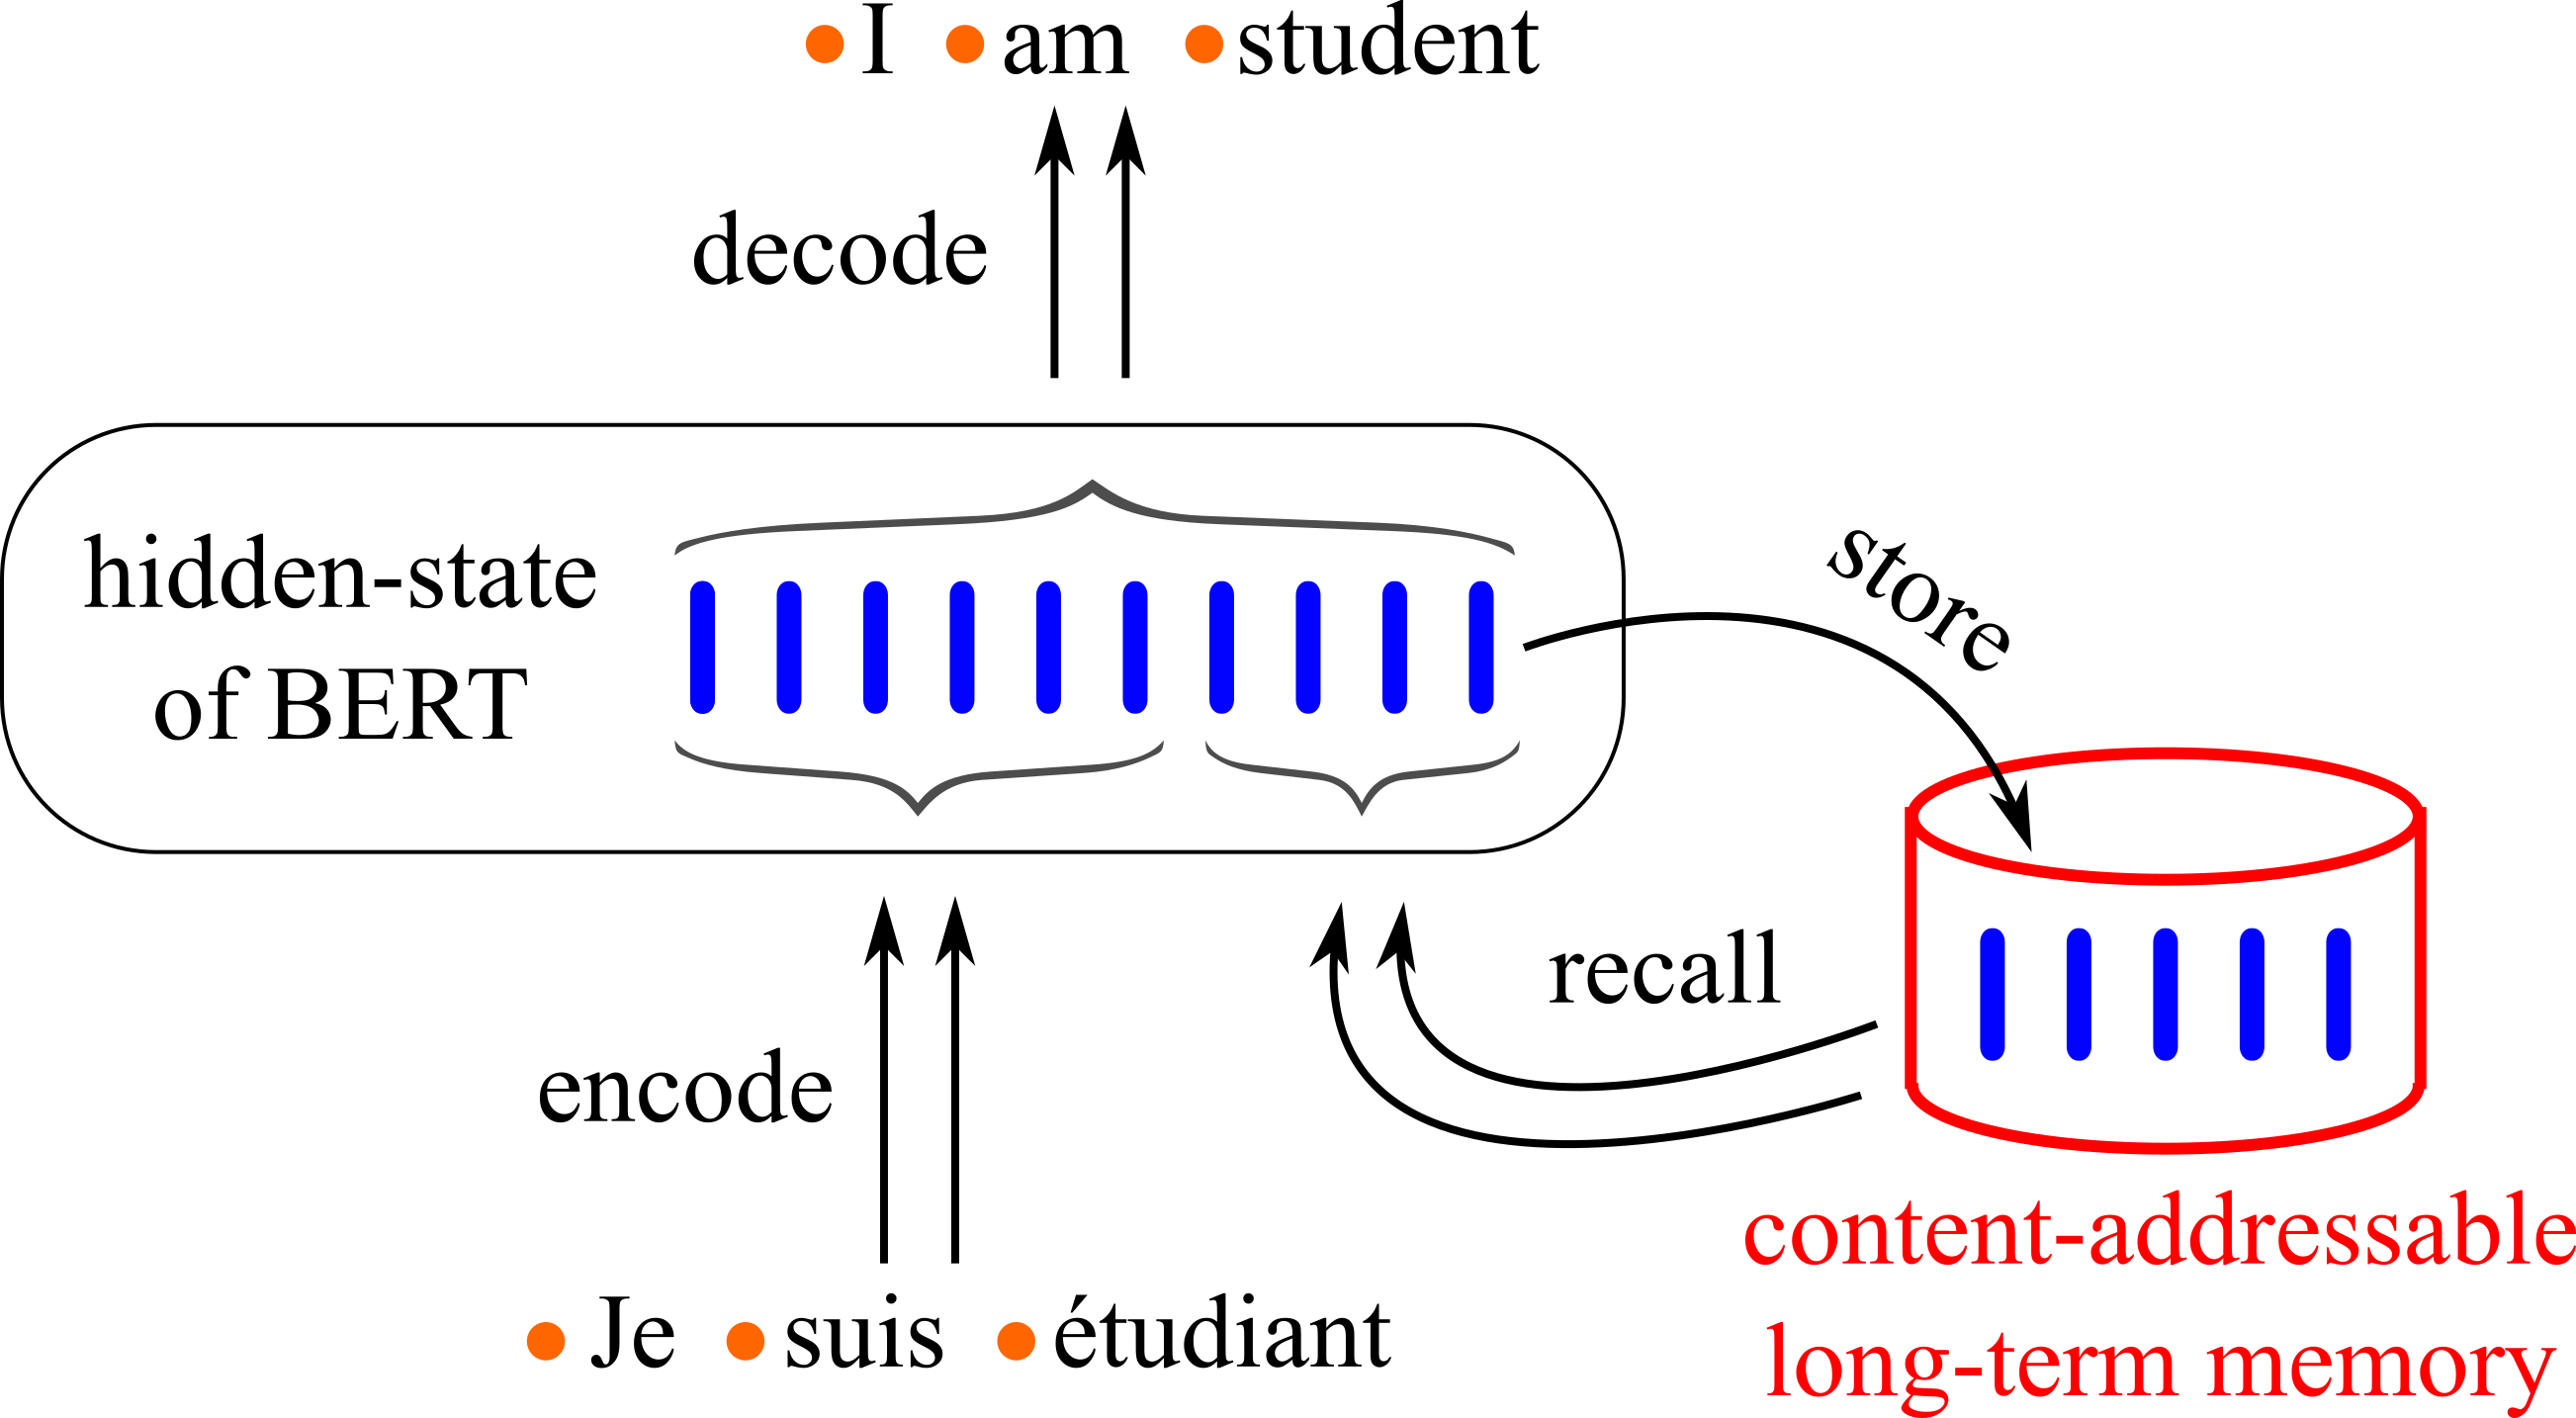
\includegraphics[scale=0.5]{long-term-memory.png}}}
	\end{equation}
	\item 这种系统 已非常接近 strong AI
	\item Content-addressable memory 的想法来自 Alex Graves \textit{et al} 的 Neural Turing Machine [2014]
	\item 以前 BERT 的隐状态 没有逻辑结构,我们不是很清楚它的内容是什么; 这是有赖 \emp{逻辑化} 才能做到的
\end{itemize}
\end{frame}

\begin{frame}
\frametitle{再谈一次 逻辑结构}
\begin{itemize}
	\item 我发现 逻辑 和 AI 之间 有很漂亮的理论
	\item 现代逻辑理论 揭示出某些 \emp{几何} (geometry) 与 \emp{拓樸} (topology) 结构
	\item 大家 中/小学 时期 都熟悉 Venn diagrams,其实 命题逻辑 具有 \emp{拓扑}结构:
	\begin{equation}
	\vcenter{\hbox{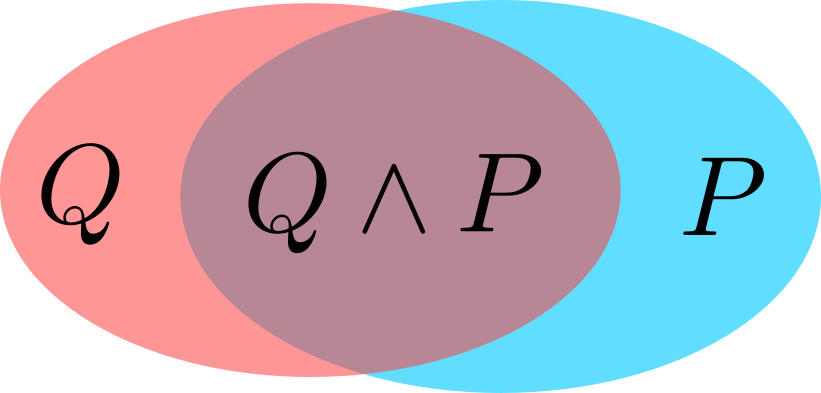
\includegraphics[scale=0.4]{Venn-diagram.png}}}
	\end{equation}
	而 谓词 (predicates) 是在 base set 上面的 纤维化 (fibration), 记作 $\mathrel{\substack{\mathbb{E}\\\downarrow \\\mathbb{B}}  {\scriptstyle p}}$

	\item 另方面,著名的 Curry-Howard isomorphism 揭示 \emp{逻辑证明} 与 \emp{编程语言} 之间的深刻关系:
	\begin{eqnarray}
	\mbox{逻辑} & \Leftrightarrow & \mbox{type theory} \\
	\mbox{逻辑证明} & \Leftrightarrow & \mbox{programs} \nonumber
	\end{eqnarray}
	\item 程式 是一些 \emp{函数},而 神经网络 也是非线性的函数\emp{映射},所以 神经网络 也\emp{对应于} 逻辑推理
\end{itemize}
\end{frame}

\begin{frame}[fragile]
\begin{itemize}
	\item BERT 似乎是在执行 句子之间的变换,而这些句子其实是 word embedding 的 concatenation 而已,例如:
	\begin{equation}
	\begin{tikzcd}[column sep = large]
	\mbox{苏格拉底} \cdot \mbox{是} \cdot \mbox{人}
	\arrow[r, "BERT"]
	& \mbox{苏格拉底} \cdot \mbox{会} \cdot \mbox{死}
	\end{tikzcd}
	\end{equation}
	这个做法看似很「粗暴」,但其实它和逻辑式子的作用一样:
	\begin{equation}
	\forall x. \; \mbox{Human}(x) \rightarrow \mbox{Mortal}(x)
	\end{equation}
	而这式子根据 Curry-Howard 对应於 上面的函数映射,这个映射保持 逻辑 predicate 的 几何/拓扑 结构

	% \item 集合元素 $a$ 是 $\exists x. P(x)$ 的证明,例如 Socrates 是 $\exists x. \mbox{mortal}(x)$ 的证明
	% \item 当 神经网络 \emp{调教} 某些元素的 映射 (mapping) 时,它同时在学习某个逻辑的 formula;  换句话说,逻辑 是几何空间中的映射
	% \item 逻辑的 谓词 (predicates) 是在 基底元素空间上的一个 \emp{纤维丛结构} (fibration) :
	%\begin{equation}
	%\vcenter{\hbox{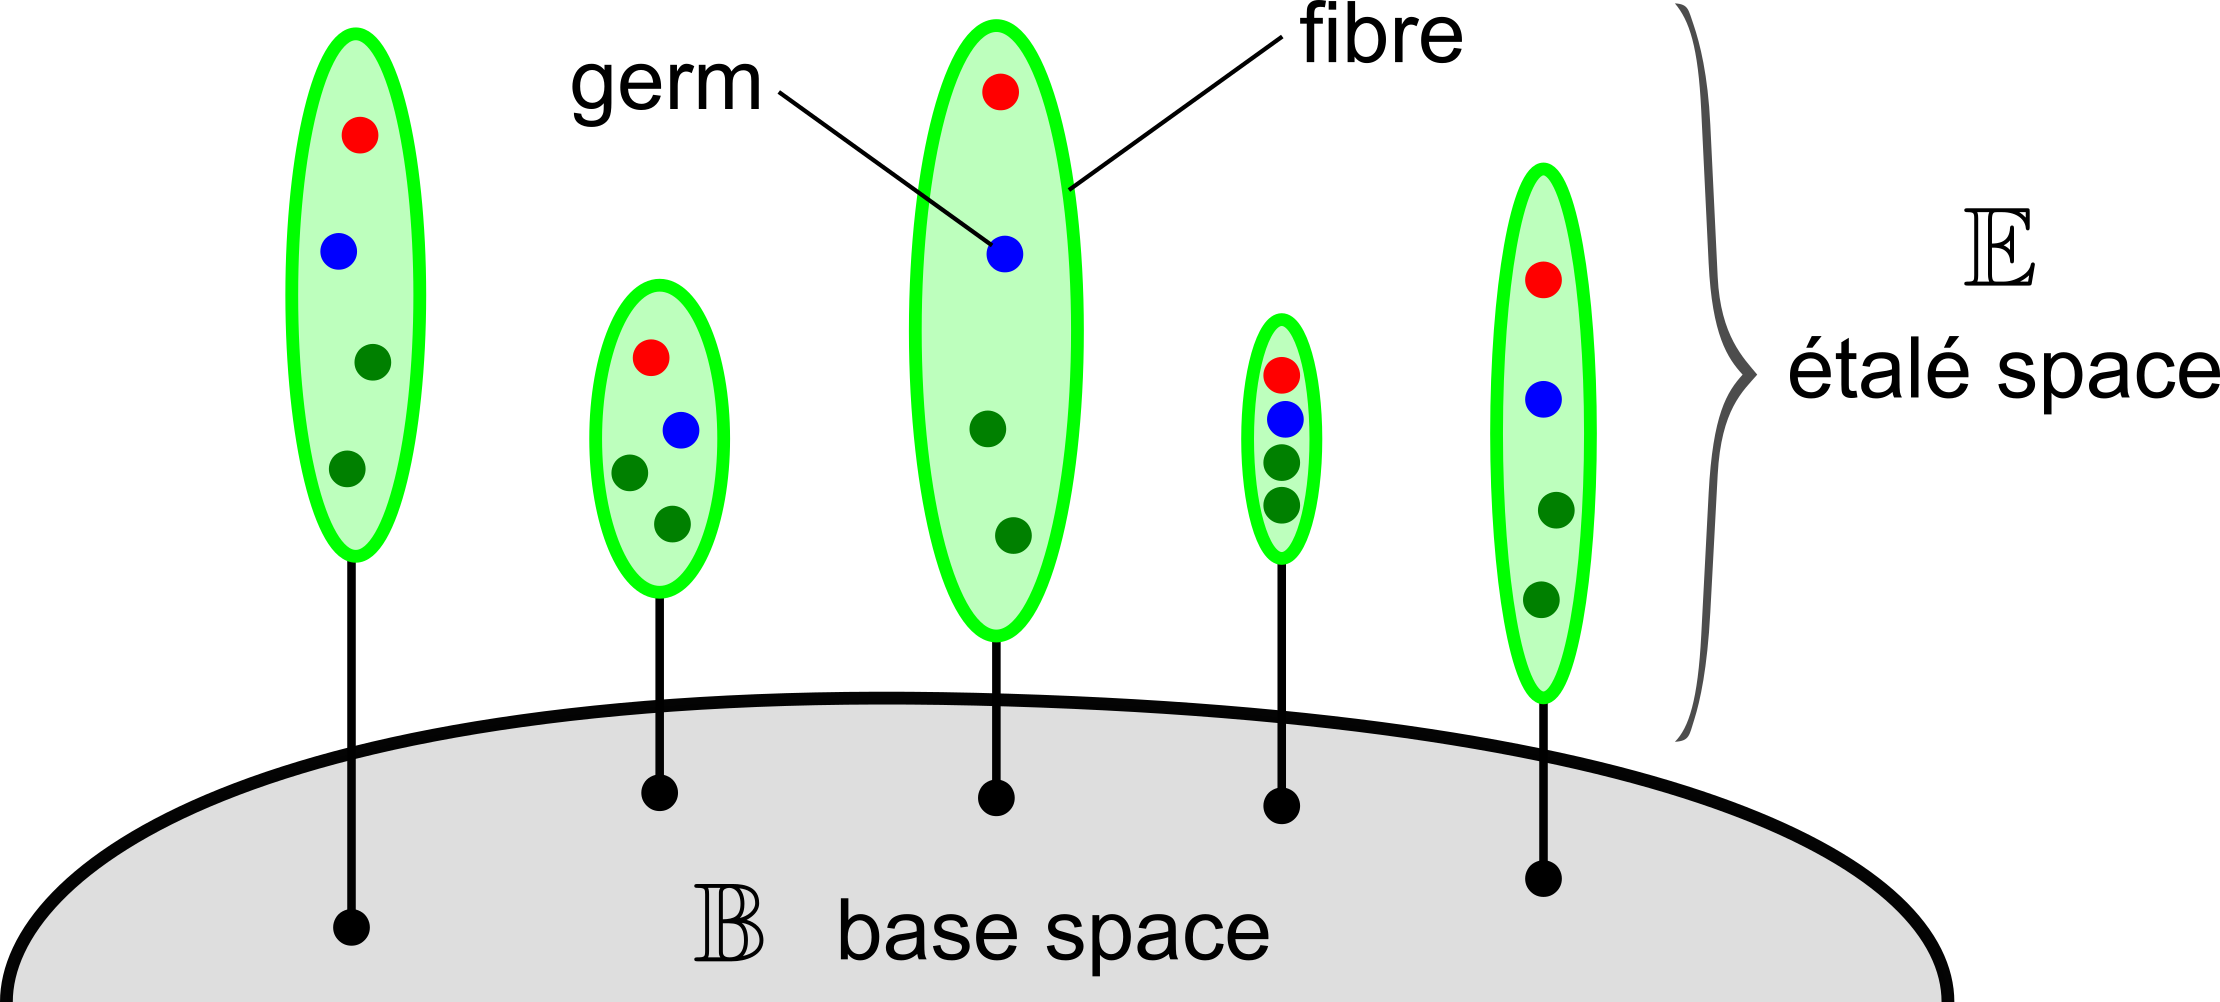
\includegraphics[scale=0.5]{etale-space.png}}}
	%\end{equation}
	\item 从 几何/拓扑 ``借'' 来的概念,演变成 topos 理论、HoTT (homotopy type theory) 等
	\item 这些漂亮的理论 不是无用的; 长远来说,它可以指导 深度学习 和 逻辑 之间的 融合,但暂时来说,我只利用了 commutativity
\end{itemize}
\end{frame}

\frameinlbffalse
\begin{frame}
\frametitle{References}
\printbibliography
\textbf{Illustration credits:}
\begin{itemize}
	\item Translation invariance, from Udacity Course 730, Deep Learning (L3 Convolutional Neural Networks $\rhd$ Convolutional Networks)
	\item \'{E}tale space, from Topoi -- The Categorical Analysis of Logic [Goldblatt 2006]
\end{itemize}
\end{frame}

\end{document} 